% ============================================================================
\section{Evaluation and responsible deployment}
% ============================================================================

% --- Source: Lecture-12 tts\_and\_vc; Columbia MCD (Works cited 37--39);
%     TTS Lecture Material Generation Request ---
\begin{frame}{Evaluating TTS quality}
  \begin{itemize}
    \item \textbf{Human tests:} Does the voice sound natural?
    \item \textbf{Similarity:} Is the generated speech close to real speech?
    \item \textbf{Intelligibility:} Can speech-to-text systems understand it?
    \item \textbf{Cloning:} How well does it copy a specific voice?
    \item TTS is evaluated by playing a sentence to human listeners and having them
give a mean opinion score (MOS) on a scale of 1 to 5.
  \end{itemize}
\end{frame}

% --- Source: Towards Responsible Evaluation for TTS (Works cited 1--3, 43);
%     Iterate to Differentiate (Works cited 36); TTS Lecture Material Generation Request ---
% \begin{frame}{Responsible evaluation (2025 framework)}
%   \begin{itemize}
%     \item \textbf{Level 1--2:} perceptual quality + robustness (bias across accents, long inputs, numbers).
%     \item \textbf{Level 3:} ethical and risk oversight---traceability, consent, legal validity of training data.
%     \item \textbf{Iterate to Differentiate (I2D):} recursive synthesis using model outputs as references to amplify failure modes.
%     \item Saturation of legacy metrics motivates more \textbf{discriminative} and \textbf{human-centered} protocols.
%   \end{itemize}
% \end{frame}

\begin{frame}{Ethics before you collect speech}
  \centering
  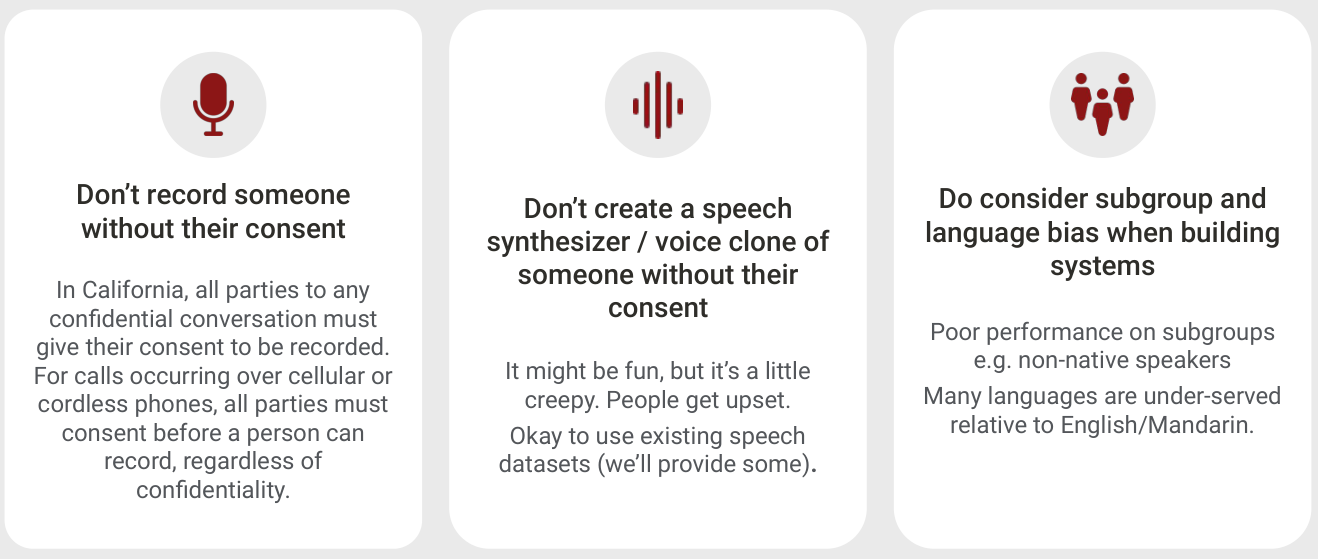
\includegraphics[width=\textwidth,height=0.62\textheight,keepaspectratio]{assets/New-Lecture-TTS/cs224s_2024_lec1/slide_08.png}
  \slideimgsource{Stanford CS224S, Lecture 1 (2024 Spring).}
\end{frame}

\begin{frame}{Takeaways}
  \begin{itemize}
    \item One text can be spoken many ways (speed, stress, intonation). Most systems still go {text $\rightarrow$ acoustic features $\rightarrow$ waveform}; newer models like VALL-E predict {audio tokens} directly.
    \item TTS improved in stages: {stitch recorded clips} $\rightarrow$ {slow but high-quality} neural models (Tacotron~2, WaveNet) $\rightarrow$ {faster parallel} models (FastSpeech~2, HiFi-GAN, VITS) $\rightarrow$ {foundation models} that clone voices from a short sample (VALL-E, Voicebox).
    \item {Voice cloning} from a few seconds of audio works well today, but can fail on rare accents; use it carefully with {consent, labeling, and fake-speech detection}.
  \end{itemize}
\end{frame}
